% Created by tikzDevice version 0.12.6 on 2024-05-23 07:11:39
% !TEX encoding = UTF-8 Unicode
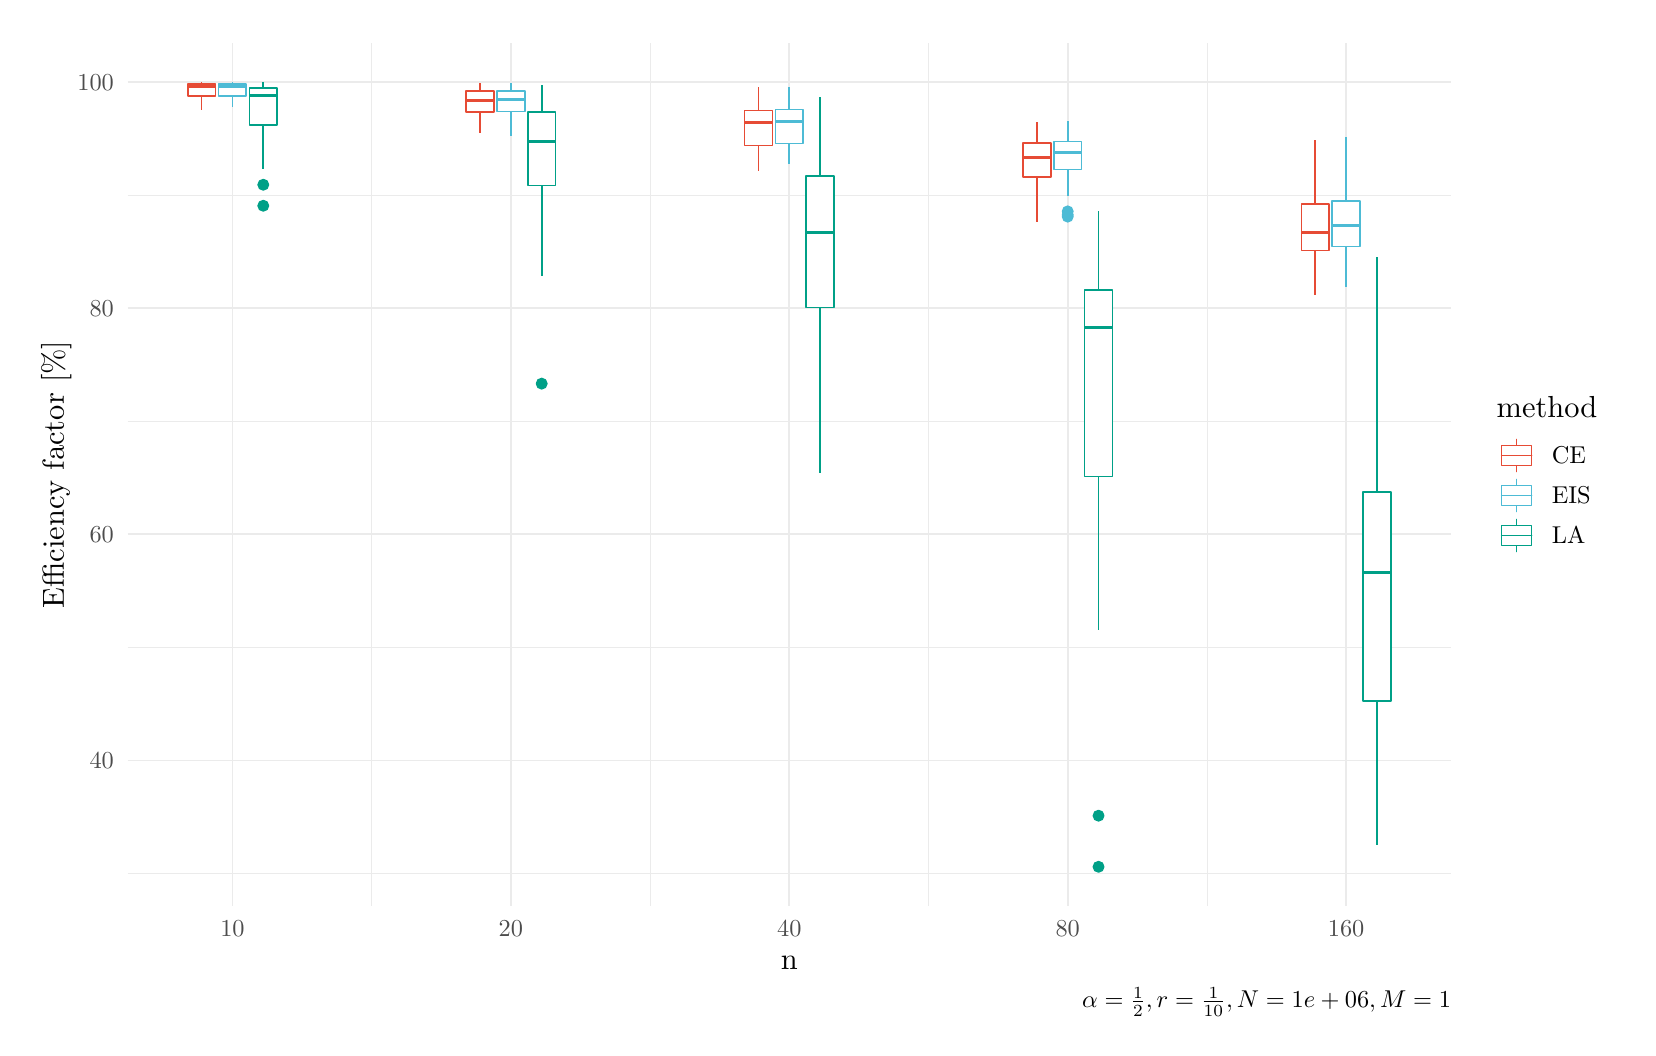
\begin{tikzpicture}[x=1pt,y=1pt]
\definecolor{fillColor}{RGB}{255,255,255}
\path[use as bounding box,fill=fillColor,fill opacity=0.00] (0,0) rectangle (578.16,361.35);
\begin{scope}
\path[clip] ( 36.11, 43.96) rectangle (514.31,355.85);
\definecolor{drawColor}{gray}{0.92}

\path[draw=drawColor,line width= 0.3pt,line join=round] ( 36.11, 55.69) --
	(514.31, 55.69);

\path[draw=drawColor,line width= 0.3pt,line join=round] ( 36.11,137.41) --
	(514.31,137.41);

\path[draw=drawColor,line width= 0.3pt,line join=round] ( 36.11,219.13) --
	(514.31,219.13);

\path[draw=drawColor,line width= 0.3pt,line join=round] ( 36.11,300.85) --
	(514.31,300.85);

\path[draw=drawColor,line width= 0.3pt,line join=round] (124.30, 43.96) --
	(124.30,355.85);

\path[draw=drawColor,line width= 0.3pt,line join=round] (224.91, 43.96) --
	(224.91,355.85);

\path[draw=drawColor,line width= 0.3pt,line join=round] (325.51, 43.96) --
	(325.51,355.85);

\path[draw=drawColor,line width= 0.3pt,line join=round] (426.12, 43.96) --
	(426.12,355.85);

\path[draw=drawColor,line width= 0.6pt,line join=round] ( 36.11, 96.55) --
	(514.31, 96.55);

\path[draw=drawColor,line width= 0.6pt,line join=round] ( 36.11,178.27) --
	(514.31,178.27);

\path[draw=drawColor,line width= 0.6pt,line join=round] ( 36.11,259.99) --
	(514.31,259.99);

\path[draw=drawColor,line width= 0.6pt,line join=round] ( 36.11,341.71) --
	(514.31,341.71);

\path[draw=drawColor,line width= 0.6pt,line join=round] ( 74.00, 43.96) --
	( 74.00,355.85);

\path[draw=drawColor,line width= 0.6pt,line join=round] (174.60, 43.96) --
	(174.60,355.85);

\path[draw=drawColor,line width= 0.6pt,line join=round] (275.21, 43.96) --
	(275.21,355.85);

\path[draw=drawColor,line width= 0.6pt,line join=round] (375.81, 43.96) --
	(375.81,355.85);

\path[draw=drawColor,line width= 0.6pt,line join=round] (476.42, 43.96) --
	(476.42,355.85);
\definecolor{drawColor}{RGB}{230,75,53}

\path[draw=drawColor,line width= 0.6pt,line join=round] ( 62.86,341.01) -- ( 62.86,341.66);

\path[draw=drawColor,line width= 0.6pt,line join=round] ( 62.86,336.69) -- ( 62.86,331.75);
\definecolor{fillColor}{RGB}{255,255,255}

\path[draw=drawColor,line width= 0.6pt,line join=round,line cap=round,fill=fillColor] ( 57.85,341.01) --
	( 57.85,336.69) --
	( 67.87,336.69) --
	( 67.87,341.01) --
	( 57.85,341.01) --
	cycle;

\path[draw=drawColor,line width= 1.1pt,line join=round] ( 57.85,340.12) -- ( 67.87,340.12);

\path[draw=drawColor,line width= 0.6pt,line join=round] (163.46,338.40) -- (163.46,341.37);

\path[draw=drawColor,line width= 0.6pt,line join=round] (163.46,330.82) -- (163.46,323.16);

\path[draw=drawColor,line width= 0.6pt,line join=round,line cap=round,fill=fillColor] (158.45,338.40) --
	(158.45,330.82) --
	(168.48,330.82) --
	(168.48,338.40) --
	(158.45,338.40) --
	cycle;

\path[draw=drawColor,line width= 1.1pt,line join=round] (158.45,335.13) -- (168.48,335.13);

\path[draw=drawColor,line width= 0.6pt,line join=round] (264.07,331.46) -- (264.07,339.99);

\path[draw=drawColor,line width= 0.6pt,line join=round] (264.07,318.74) -- (264.07,309.56);

\path[draw=drawColor,line width= 0.6pt,line join=round,line cap=round,fill=fillColor] (259.06,331.46) --
	(259.06,318.74) --
	(269.08,318.74) --
	(269.08,331.46) --
	(259.06,331.46) --
	cycle;

\path[draw=drawColor,line width= 1.1pt,line join=round] (259.06,326.98) -- (269.08,326.98);

\path[draw=drawColor,line width= 0.6pt,line join=round] (364.67,319.65) -- (364.67,327.22);

\path[draw=drawColor,line width= 0.6pt,line join=round] (364.67,307.33) -- (364.67,291.16);

\path[draw=drawColor,line width= 0.6pt,line join=round,line cap=round,fill=fillColor] (359.66,319.65) --
	(359.66,307.33) --
	(369.69,307.33) --
	(369.69,319.65) --
	(359.66,319.65) --
	cycle;

\path[draw=drawColor,line width= 1.1pt,line join=round] (359.66,314.31) -- (369.69,314.31);

\path[draw=drawColor,line width= 0.6pt,line join=round] (465.28,297.61) -- (465.28,320.79);

\path[draw=drawColor,line width= 0.6pt,line join=round] (465.28,280.81) -- (465.28,264.78);

\path[draw=drawColor,line width= 0.6pt,line join=round,line cap=round,fill=fillColor] (460.27,297.61) --
	(460.27,280.81) --
	(470.29,280.81) --
	(470.29,297.61) --
	(460.27,297.61) --
	cycle;

\path[draw=drawColor,line width= 1.1pt,line join=round] (460.27,287.25) -- (470.29,287.25);
\definecolor{drawColor}{RGB}{77,187,213}

\path[draw=drawColor,line width= 0.6pt,line join=round] ( 74.00,341.03) -- ( 74.00,341.67);

\path[draw=drawColor,line width= 0.6pt,line join=round] ( 74.00,336.77) -- ( 74.00,332.69);

\path[draw=drawColor,line width= 0.6pt,line join=round,line cap=round,fill=fillColor] ( 68.99,341.03) --
	( 68.99,336.77) --
	( 79.01,336.77) --
	( 79.01,341.03) --
	( 68.99,341.03) --
	cycle;

\path[draw=drawColor,line width= 1.1pt,line join=round] ( 68.99,340.14) -- ( 79.01,340.14);

\path[draw=drawColor,line width= 0.6pt,line join=round] (174.60,338.47) -- (174.60,341.40);

\path[draw=drawColor,line width= 0.6pt,line join=round] (174.60,331.05) -- (174.60,322.36);

\path[draw=drawColor,line width= 0.6pt,line join=round,line cap=round,fill=fillColor] (169.59,338.47) --
	(169.59,331.05) --
	(179.62,331.05) --
	(179.62,338.47) --
	(169.59,338.47) --
	cycle;

\path[draw=drawColor,line width= 1.1pt,line join=round] (169.59,335.30) -- (179.62,335.30);

\path[draw=drawColor,line width= 0.6pt,line join=round] (275.21,331.74) -- (275.21,340.03);

\path[draw=drawColor,line width= 0.6pt,line join=round] (275.21,319.48) -- (275.21,312.11);

\path[draw=drawColor,line width= 0.6pt,line join=round,line cap=round,fill=fillColor] (270.20,331.74) --
	(270.20,319.48) --
	(280.22,319.48) --
	(280.22,331.74) --
	(270.20,331.74) --
	cycle;

\path[draw=drawColor,line width= 1.1pt,line join=round] (270.20,327.46) -- (280.22,327.46);
\definecolor{fillColor}{RGB}{77,187,213}

\path[draw=drawColor,line width= 0.4pt,line join=round,line cap=round,fill=fillColor] (375.81,293.07) circle (  1.96);

\path[draw=drawColor,line width= 0.4pt,line join=round,line cap=round,fill=fillColor] (375.81,293.75) circle (  1.96);

\path[draw=drawColor,line width= 0.4pt,line join=round,line cap=round,fill=fillColor] (375.81,294.96) circle (  1.96);

\path[draw=drawColor,line width= 0.6pt,line join=round] (375.81,320.19) -- (375.81,327.51);

\path[draw=drawColor,line width= 0.6pt,line join=round] (375.81,310.13) -- (375.81,300.42);
\definecolor{fillColor}{RGB}{255,255,255}

\path[draw=drawColor,line width= 0.6pt,line join=round,line cap=round,fill=fillColor] (370.80,320.19) --
	(370.80,310.13) --
	(380.83,310.13) --
	(380.83,320.19) --
	(370.80,320.19) --
	cycle;

\path[draw=drawColor,line width= 1.1pt,line join=round] (370.80,316.10) -- (380.83,316.10);

\path[draw=drawColor,line width= 0.6pt,line join=round] (476.42,298.79) -- (476.42,321.86);

\path[draw=drawColor,line width= 0.6pt,line join=round] (476.42,282.23) -- (476.42,267.48);

\path[draw=drawColor,line width= 0.6pt,line join=round,line cap=round,fill=fillColor] (471.41,298.79) --
	(471.41,282.23) --
	(481.43,282.23) --
	(481.43,298.79) --
	(471.41,298.79) --
	cycle;

\path[draw=drawColor,line width= 1.1pt,line join=round] (471.41,289.81) -- (481.43,289.81);
\definecolor{drawColor}{RGB}{0,160,135}
\definecolor{fillColor}{RGB}{0,160,135}

\path[draw=drawColor,line width= 0.4pt,line join=round,line cap=round,fill=fillColor] ( 85.14,297.00) circle (  1.96);

\path[draw=drawColor,line width= 0.4pt,line join=round,line cap=round,fill=fillColor] ( 85.14,304.59) circle (  1.96);

\path[draw=drawColor,line width= 0.6pt,line join=round] ( 85.14,339.62) -- ( 85.14,341.54);

\path[draw=drawColor,line width= 0.6pt,line join=round] ( 85.14,326.19) -- ( 85.14,310.43);
\definecolor{fillColor}{RGB}{255,255,255}

\path[draw=drawColor,line width= 0.6pt,line join=round,line cap=round,fill=fillColor] ( 80.13,339.62) --
	( 80.13,326.19) --
	( 90.15,326.19) --
	( 90.15,339.62) --
	( 80.13,339.62) --
	cycle;

\path[draw=drawColor,line width= 1.1pt,line join=round] ( 80.13,336.95) -- ( 90.15,336.95);
\definecolor{fillColor}{RGB}{0,160,135}

\path[draw=drawColor,line width= 0.4pt,line join=round,line cap=round,fill=fillColor] (185.74,232.72) circle (  1.96);

\path[draw=drawColor,line width= 0.6pt,line join=round] (185.74,330.86) -- (185.74,340.57);

\path[draw=drawColor,line width= 0.6pt,line join=round] (185.74,304.34) -- (185.74,271.66);
\definecolor{fillColor}{RGB}{255,255,255}

\path[draw=drawColor,line width= 0.6pt,line join=round,line cap=round,fill=fillColor] (180.73,330.86) --
	(180.73,304.34) --
	(190.76,304.34) --
	(190.76,330.86) --
	(180.73,330.86) --
	cycle;

\path[draw=drawColor,line width= 1.1pt,line join=round] (180.73,320.27) -- (190.76,320.27);

\path[draw=drawColor,line width= 0.6pt,line join=round] (286.35,307.70) -- (286.35,336.29);

\path[draw=drawColor,line width= 0.6pt,line join=round] (286.35,260.27) -- (286.35,200.32);

\path[draw=drawColor,line width= 0.6pt,line join=round,line cap=round,fill=fillColor] (281.34,307.70) --
	(281.34,260.27) --
	(291.36,260.27) --
	(291.36,307.70) --
	(281.34,307.70) --
	cycle;

\path[draw=drawColor,line width= 1.1pt,line join=round] (281.34,287.16) -- (291.36,287.16);
\definecolor{fillColor}{RGB}{0,160,135}

\path[draw=drawColor,line width= 0.4pt,line join=round,line cap=round,fill=fillColor] (386.95, 76.60) circle (  1.96);

\path[draw=drawColor,line width= 0.4pt,line join=round,line cap=round,fill=fillColor] (386.95, 58.13) circle (  1.96);

\path[draw=drawColor,line width= 0.6pt,line join=round] (386.95,266.60) -- (386.95,295.26);

\path[draw=drawColor,line width= 0.6pt,line join=round] (386.95,199.19) -- (386.95,143.60);
\definecolor{fillColor}{RGB}{255,255,255}

\path[draw=drawColor,line width= 0.6pt,line join=round,line cap=round,fill=fillColor] (381.94,266.60) --
	(381.94,199.19) --
	(391.97,199.19) --
	(391.97,266.60) --
	(381.94,266.60) --
	cycle;

\path[draw=drawColor,line width= 1.1pt,line join=round] (381.94,252.87) -- (391.97,252.87);

\path[draw=drawColor,line width= 0.6pt,line join=round] (487.56,193.63) -- (487.56,278.42);

\path[draw=drawColor,line width= 0.6pt,line join=round] (487.56,118.11) -- (487.56, 66.01);

\path[draw=drawColor,line width= 0.6pt,line join=round,line cap=round,fill=fillColor] (482.55,193.63) --
	(482.55,118.11) --
	(492.57,118.11) --
	(492.57,193.63) --
	(482.55,193.63) --
	cycle;

\path[draw=drawColor,line width= 1.1pt,line join=round] (482.55,164.44) -- (492.57,164.44);
\end{scope}
\begin{scope}
\path[clip] (  0.00,  0.00) rectangle (578.16,361.35);
\definecolor{drawColor}{gray}{0.30}

\node[text=drawColor,anchor=base east,inner sep=0pt, outer sep=0pt, scale=  0.88] at ( 31.16, 93.52) {40};

\node[text=drawColor,anchor=base east,inner sep=0pt, outer sep=0pt, scale=  0.88] at ( 31.16,175.24) {60};

\node[text=drawColor,anchor=base east,inner sep=0pt, outer sep=0pt, scale=  0.88] at ( 31.16,256.96) {80};

\node[text=drawColor,anchor=base east,inner sep=0pt, outer sep=0pt, scale=  0.88] at ( 31.16,338.68) {100};
\end{scope}
\begin{scope}
\path[clip] (  0.00,  0.00) rectangle (578.16,361.35);
\definecolor{drawColor}{gray}{0.30}

\node[text=drawColor,anchor=base,inner sep=0pt, outer sep=0pt, scale=  0.88] at ( 74.00, 32.95) {10};

\node[text=drawColor,anchor=base,inner sep=0pt, outer sep=0pt, scale=  0.88] at (174.60, 32.95) {20};

\node[text=drawColor,anchor=base,inner sep=0pt, outer sep=0pt, scale=  0.88] at (275.21, 32.95) {40};

\node[text=drawColor,anchor=base,inner sep=0pt, outer sep=0pt, scale=  0.88] at (375.81, 32.95) {80};

\node[text=drawColor,anchor=base,inner sep=0pt, outer sep=0pt, scale=  0.88] at (476.42, 32.95) {160};
\end{scope}
\begin{scope}
\path[clip] (  0.00,  0.00) rectangle (578.16,361.35);
\definecolor{drawColor}{RGB}{0,0,0}

\node[text=drawColor,anchor=base,inner sep=0pt, outer sep=0pt, scale=  1.10] at (275.21, 20.91) {n};
\end{scope}
\begin{scope}
\path[clip] (  0.00,  0.00) rectangle (578.16,361.35);
\definecolor{drawColor}{RGB}{0,0,0}

\node[text=drawColor,rotate= 90.00,anchor=base,inner sep=0pt, outer sep=0pt, scale=  1.10] at ( 13.08,199.90) {Efficiency factor [\%]};
\end{scope}
\begin{scope}
\path[clip] (  0.00,  0.00) rectangle (578.16,361.35);
\definecolor{drawColor}{RGB}{0,0,0}

\node[text=drawColor,anchor=base west,inner sep=0pt, outer sep=0pt, scale=  1.10] at (530.81,220.55) {method};
\end{scope}
\begin{scope}
\path[clip] (  0.00,  0.00) rectangle (578.16,361.35);
\definecolor{drawColor}{RGB}{230,75,53}

\path[draw=drawColor,line width= 0.6pt,line join=round,line cap=round] (538.03,200.97) --
	(538.03,203.14);

\path[draw=drawColor,line width= 0.6pt,line join=round,line cap=round] (538.03,210.36) --
	(538.03,212.53);
\definecolor{fillColor}{RGB}{255,255,255}

\path[draw=drawColor,line width= 0.6pt,line join=round,line cap=round,fill=fillColor] (532.61,203.14) rectangle (543.45,210.36);

\path[draw=drawColor,line width= 0.6pt,line join=round,line cap=round] (532.61,206.75) --
	(543.45,206.75);
\end{scope}
\begin{scope}
\path[clip] (  0.00,  0.00) rectangle (578.16,361.35);
\definecolor{drawColor}{RGB}{77,187,213}

\path[draw=drawColor,line width= 0.6pt,line join=round,line cap=round] (538.03,186.51) --
	(538.03,188.68);

\path[draw=drawColor,line width= 0.6pt,line join=round,line cap=round] (538.03,195.91) --
	(538.03,198.08);
\definecolor{fillColor}{RGB}{255,255,255}

\path[draw=drawColor,line width= 0.6pt,line join=round,line cap=round,fill=fillColor] (532.61,188.68) rectangle (543.45,195.91);

\path[draw=drawColor,line width= 0.6pt,line join=round,line cap=round] (532.61,192.30) --
	(543.45,192.30);
\end{scope}
\begin{scope}
\path[clip] (  0.00,  0.00) rectangle (578.16,361.35);
\definecolor{drawColor}{RGB}{0,160,135}

\path[draw=drawColor,line width= 0.6pt,line join=round,line cap=round] (538.03,172.06) --
	(538.03,174.23);

\path[draw=drawColor,line width= 0.6pt,line join=round,line cap=round] (538.03,181.46) --
	(538.03,183.62);
\definecolor{fillColor}{RGB}{255,255,255}

\path[draw=drawColor,line width= 0.6pt,line join=round,line cap=round,fill=fillColor] (532.61,174.23) rectangle (543.45,181.46);

\path[draw=drawColor,line width= 0.6pt,line join=round,line cap=round] (532.61,177.84) --
	(543.45,177.84);
\end{scope}
\begin{scope}
\path[clip] (  0.00,  0.00) rectangle (578.16,361.35);
\definecolor{drawColor}{RGB}{0,0,0}

\node[text=drawColor,anchor=base west,inner sep=0pt, outer sep=0pt, scale=  0.88] at (550.76,203.72) {CE};
\end{scope}
\begin{scope}
\path[clip] (  0.00,  0.00) rectangle (578.16,361.35);
\definecolor{drawColor}{RGB}{0,0,0}

\node[text=drawColor,anchor=base west,inner sep=0pt, outer sep=0pt, scale=  0.88] at (550.76,189.27) {EIS};
\end{scope}
\begin{scope}
\path[clip] (  0.00,  0.00) rectangle (578.16,361.35);
\definecolor{drawColor}{RGB}{0,0,0}

\node[text=drawColor,anchor=base west,inner sep=0pt, outer sep=0pt, scale=  0.88] at (550.76,174.81) {LA};
\end{scope}
\begin{scope}
\path[clip] (  0.00,  0.00) rectangle (578.16,361.35);
\definecolor{drawColor}{RGB}{0,0,0}

\node[text=drawColor,anchor=base east,inner sep=0pt, outer sep=0pt, scale=  0.88] at (514.31,  7.21) {$\alpha = \frac 1 2, r = \frac 1 {10}, N = 1e+06, M=1$};
\end{scope}
\end{tikzpicture}
